\chapter{\label{chp:lartpcs} Liquid Argon Time Projection Chambers}

\section{Time Projection Chambers}

The Time Projection Chamber, abbreviated TPC, is a revolutionary particle detector concept first proposed in 1974 by David Nygren at Lawrence Berkeley National Lab.  Since then, the TPC has found applications in a broad array of particle physics experiments such as collider experiments at the LHC \cite{Lippmann:2104844,Aamodt:2008zz}, precision measurements of muon properties \cite{Luo:2015oca}, dark matter experiments \cite{Akerib:2012ys,Aprile:2011dd} and more.  The abundance of uses for the TPC technology stems from the versatile and robust ability of a TPC to track charged particles.

In general, a Time Projection Chamber is a volume filled with some neutral and inert material.  Commonly, noble gases and liquids are used though this is not required.  An electric field is applied to the entire medium, and in some cases a magnetic field is applied as well.  The electric field is generally applied by using a high voltage cathode as one surface of the detector.  The opposing surface, the anode, is typically instrumented with readout equipment.

Time Projection Chambers are designed to observe electrically charged particles.  In particular, a high energy charged particle (such as an electron, muon, pion, proton, etc.) can travel through the detector medium and will ionize the substance as it passes through, leaving a trail of electrons and ions.  The applied electric field, emanating from the cathode, serves to separate the ionization electrons from the ions and move the electrons towards the anode of the detector.  The drifted electrons form the basis of the measurement of the particle.  In particular, they appear as a projection of the original track onto the anode of the detector, and the distance from the anode is determined by the time it took for the electrons to drift.  Hence the name, Time Projection Chamber.

\section{History and Liquid Argon Time Projection Chamber Concepts}

The Liquid Argon Time Projection Chamber (LArTPC) was invented in 1974 by Bill Willis and Veljko Radika \cite{Willis:1974gi}, and initially proposed for neutrino physics in 1977 by Carlo Rubbia \cite{Rubbia:1977zz}.  At the time of its conception, neutrino physics was dominated by bubble chamber detectors like Gargamelle \cite{Musset:1978gf}, renowned for it's remarkable resolution of particle topologies.  Initially, the LArTPC was proposed as a way to combine high spatial resolution detectors with calorimetry measuring detectors in a way that is scalable to massive detectors.  As the field of neutrino physics approaches the largest LArTPC to date with DUNE \cite{DUNE}, it's worthwhile to recall the original advantages of the LArTPC technology as laid out in 1977 \cite{Rubbia:1977zz}:

\begin{itemize}

\item{\bf ``It is dense''}: The relatively high density of liquid argon, at 1.4 $g/cm^3$, provides a sufficiently high neutrino interaction rate such that high statistics measurements are feasible.

\item{\bf ``It does not attach electrons and permits long drift times''}: As a long drift time is essential to large scale detectors to both maximize the mass of the detector and minimize the number of readout channels, the fact that argon itself does not attach free electrons is an essential ingredient to LArTPCs.

\item{\bf ``It has a high electron mobility''}: The high mobility makes drifting electrons from particle ionization in a short time a feasible task.

\item{\bf ``It is cheap''}:  A detector can not be scaled to massive sizes unless the fundamental building block of the detector is affordable.

\item{\bf ``It is easy to obtain and purify''}: Purification challenges have largely been overcome for LArTPCs.  In particular, the \uboone experiment has demonstrated a viable way to achieve high purity argon without purging the detector of impurities first.

\item{\bf ``It is inert and can be liquified with liquid nitrogen''}: This makes the cryogenic systems for LArTPCs reasonable to purchase and implement.

\end{itemize}

40 years after the original proposal, it is remarkable how relevant the initial advantages remain in the face of an experiment such as DUNE. 

Since the original proposal, some additional advantages of LArTPCs have been noted and are worth mentioning.  For example, the scintillation of Liquid Argon has been successfully characterized \cite{Heindl:2010zz} and is measurable in coincidence with the drift ionization.  For large detectors, especially surface detectors, this allows the ability to match scintillation light to ionization tracks to reject out of time events such as cosmic particles.  It also allows the implementation of a hardware based trigger to filter neutrino interactions online.  For even modest sized LArTPCs, this can be an essential aspect to control data rates and ease computing requirements.

\section{Design of LArTPCs}
\label{sec:argoneut_detector}

As mentioned above, the Liquid Argon TPC has a long history of development.  This section presents the details of a modern LArTPC in it's design, given in the context of the \argoneut detector. A comprehensive and detailed description of the \argoneut detector is given in \cite{Anderson:2012vc}.

\subsection{\argoneut Time Projection Chamber}

The \argoneut experiment was the first \lartpc in a neutrino beam in the U.S., the first \lartpc in a low energy neutrino beam ever, and the start of the Fermilab and U.S. \lartpc program.  It was initially proposed as a test experiment to study the performance of a \lartpc in a neutrino beam, but has since produced a number of critical physics papers that were firsts of their kind.  \argoneut made the first measurements of muon neutrino cross sections on argon \cite{Anderson:2011ce, Acciarri:2014isz}, it characterized the response of the detector to several types of particles \cite{Anderson:2012mra, Acciarri:2013met}, and has made high impact measurements of short-range correlated pairs and back to back protons \cite{Acciarri:2014gev}, and coherent pion production \cite{Acciarri:2014eit}.

The \argoneut TPC is a rectangular volume of liquid argon that measures 40 cm high (Y direction), 47 cm wide (X direction), and 90 cm long (Z direction).  In total, this corresponds to about 170 liters of Liquid Argon.  In its running configuration, neutrinos from Fermilab's NuMI beam (See Section~\ref{sec:numi_beam}) enter nearly parallel to the Z direction, with a slight downward direction.  On the left side of the detector in the beam direction is the high voltage cathode, providing a uniform electric field of 500 V/cm throughout the TPC (corresponding to approximately -23 kV of voltage at the cathode).  Opposite the cathode is the anode, composed of three wire planes, of which only two are instrumented for readout.

\begin{figure}[htbp]
  \centering
  \includegraphics[width=0.75\textwidth]{lartpc_figures/argoneut_tpc_and_cryostat.pdf}
  \caption[The \argoneut TPC]{The \argoneut TPC positioned just outside of its cryostat.  The wire planes and the readout electronics are visible on the right side of the TPC.}
  \label{fig:argoneut_tpc}
\end{figure}

In the detector, as a neutrino interacts it produces outgoing particles, most commonly: muons, protons, neutrons, pions (charged and neutral), photons and electrons.  Naturally, the possible particles produced in a neutrino interaction is much broader than this short list, but this comprises some of the most frequent particles.  In the case of the electrically charged particles, the particle will ionize the argon atoms as it moves through the detector.  The ionization produced is a statistical quantity, but the average expected ionization depends strongly on the momentum and mass of the particle in question.  In general, particles with higher mass and lower momentum produce larger ionization per unit distance traveled \cite{Kalinovsky:1989kk}.  The ionization per unit distance, measured most frequently in the units MeV/cm, is a very powerful tool for calorimetric identification of particles (as demonstrated in Chapter \ref{chp:emshowers}).

Neutral particles, such as neutrons and photons, do not ionize the argon atoms as they traverse the detector.  However, these particles can still interact with the argon and produce charged particles visible to the TPC instrumentation.  Neutrons frequently will scatter off of an argon nucleus and produce a recoiling proton, which can be observed in the detector.  Photons can produce electromagnetic showers through Compton scattering and pair production, described more fully in Chapter \ref{chp:emshowers}.

After the particles from the neutrino interaction have produced ionization in the detector, the electric field separates the ions and electrons from each other.  The separation is imperfect and depends on the strength of the electric field, the amount of ionization, as well as the angle of ionization with respect to the field.  This effect, known as recombination of electrons and ions, has been studied in detail in the \argoneut detector \cite{Acciarri:2013met}.  In general, this effect causes a quenching of the observed electrons compared to the true ionizing power of the high energy particles as seen in Figure \ref{fig:argoneut_recombination}.

\begin{figure}[htbp]
  \centering
  \includegraphics[width=0.5\textwidth]{lartpc_figures/recombination_dqdx_dedx.pdf}
  \caption[\argoneut Recombination]{Measurement of the recombination effect in \argoneut using stopping protons, at 500 V/cm. \cite{Acciarri:2013met}}
  \label{fig:argoneut_recombination}
\end{figure}

The uniformity of the electric field in the \argoneut detector is maintained with a system of field shaping electrodes.  The electrodes are plated on to the interior surface of the volume between the cathode and anode, and are held at a voltage linearly decreasing from cathode to anode.  In \argoneut, the field shaping strips are 1cm wide and separated by 1cm, and there are 23 strips total.  This technique, however, is utilized in a variety of TPC experiments.

Once the electrons have been separated from the ions, they drift towards the readout wires of the TPC.  Though argon itself does not attach electrons, impurities in the argon can do so.  The amount of drifting electrons declines as a function of the distance they have to drift.  This decline is well modeled with an exponential decline, and the decay constant is referred to as the electron ``lifetime.'' Proper calorimetry must take the lifetime of the electrons into account on hit by hit basis to correctly account for the effect of the impurities in the liquid argon.  In \argoneut, the electron lifetime is measured in data by comparing the amplitude of hits from crossing muons at different drift distances as seen in Figure \ref{fig:argoneut_lifetime}.

\begin{figure}[htbp]
  \centering
  \includegraphics[width=0.5\textwidth]{lartpc_figures/argoneut_lifetime.pdf}
  \caption[\argoneut Lifetime Measurement]{The electron lifetime in \argoneut is computed run by run empirically, using a sample of depositions in the TPC from minimally ionizing particles.  Shown here is the fit, using an exponential, for run 648 giving an electron lifetime of 742 $\pm \mu$s (statistical error only).}
  \label{fig:argoneut_lifetime}
\end{figure}



The \argoneut detector has three planes of wires at the anode, two of which are instrumented.  The first plane, composed of 225 wires oriented vertically, serves as a shielding plane for the other wires and to provide shaping to the electric field through the TPC.  The three planes are spaced with 4 mm between each other.  The second plane, referred to as the ``induction plane,'' contains wires that are set at +60$^\text{o}$ to the beam axis.  As electrons cross the shield plane, they approach the induction plane wires.  The wires are electrically biased, however, such that the electrons drift around the individual wires.  The approaching and subsequent passing of electrons induces a current on these wires (hence the name ``induction plane'') and the bipolar pulse shape is recorded by the readout electronics for wires that observe electrons.  See figure \ref{fig:argoneut_signals} for examples of this pulse.

The final set of wires, dubbed the ``collection plane,'' is biased such that it collects the drifting electrons onto it and they are observed as a pulse of charge by the electronics system.  The collection plane is set at an angle of -60$^\text{o}$ to the beam direction.  The two instrumented planes each have wire spacings of 4mm, and sample at 5.05 MHz.  In total, the instrumented planes have 240 wires in each plane.  Since the wires are at an angle with respect to the TPC axes, not all wires are of the same length.  Most wires, 144 of 240 in each plane, are 46.2 cm long.  The shortest wires are 3.7 cm long.

The sense wires are readout with a system of electronics sampled every 198 ns, and the readout system has a sensitivty of 7.49 ADC/fC of charge recorded.  This gives a signal to noise ratio of 15 or higher for minimally ionizing particles in the TPC.  An in depth description of the \argoneut readout electronics is available in \cite{Anderson:2012vc}


\begin{figure}[htbp]
  \centering
  \includegraphics[width=\textwidth]{lartpc_figures/argoneut_signal.pdf}
  \caption[Deconvolution of \argoneut Signals]{Raw and deconvoluted signal shapes from the \argoneut detector.  On the top is shown the induction pulse.  The bipolar shape of the pulse in the induction plane is corrected during the deconvolution stage.  On both planes, a Gaussian hit fitting technique is used to determine the amount of charge recorded. Figure from \cite{Anderson:2012vc}.}
  \label{fig:argoneut_signals}
\end{figure}

\section{\label{sec:lartpc_reconstruction} Event Imaging and Reconstruction}

One of the prime advantages of a \lartpc to other neutrino detection technologies is the ability to do precision imaging {\em and} calorimetry.  In this section, the standard chain of reconstruction algorithms is described to show how the high resolution images are transformed into high level, particle physics data.

Each wire in the detector measures a signal of electrons as they drift, as a function of time.  When the wires are arrayed in an image in sequential order, such that the x axis is wire number and the y axis is time tick, 2D images are formed such as in figure \ref{fig:argoneut_data}.  As seen in figure \ref{fig:argoneut_projection}, the wire planes represent projections of the 3D data onto a plane that is orthogonal to the wires themselves.

\begin{figure}[htbp]
  \centering
  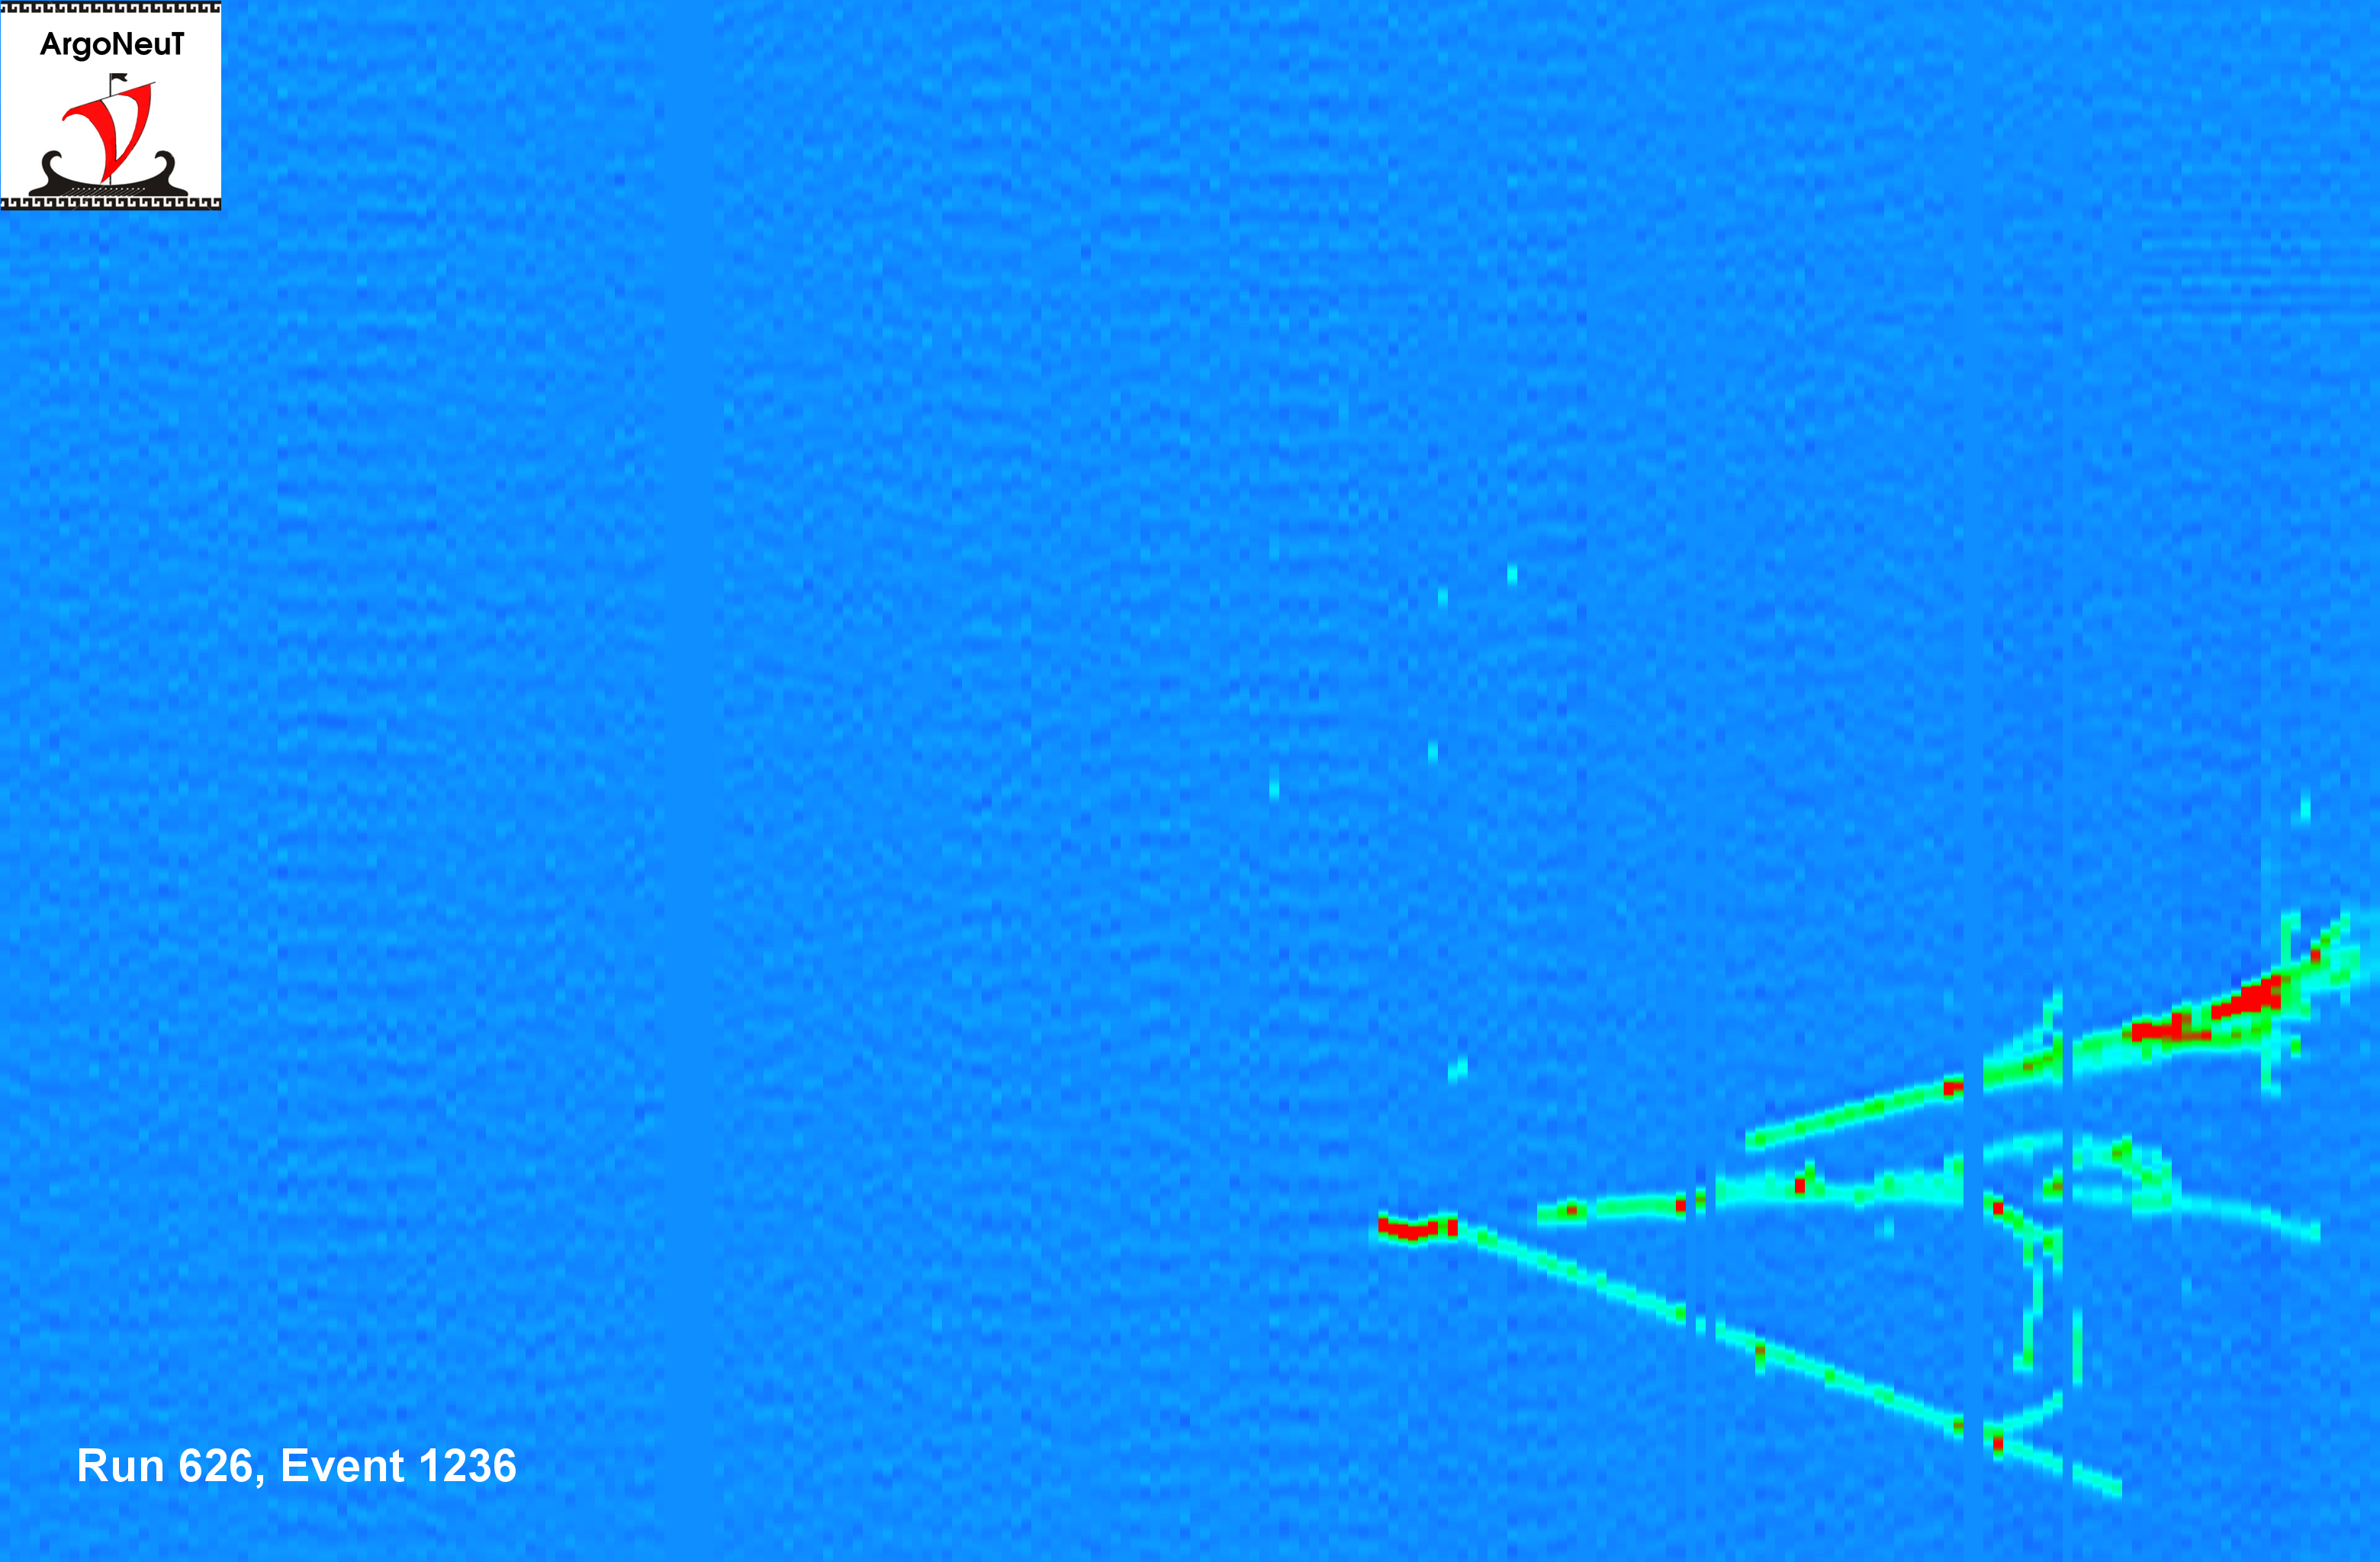
\includegraphics[width=0.85\textwidth]{lartpc_figures/R626_E1236_collection.png}
  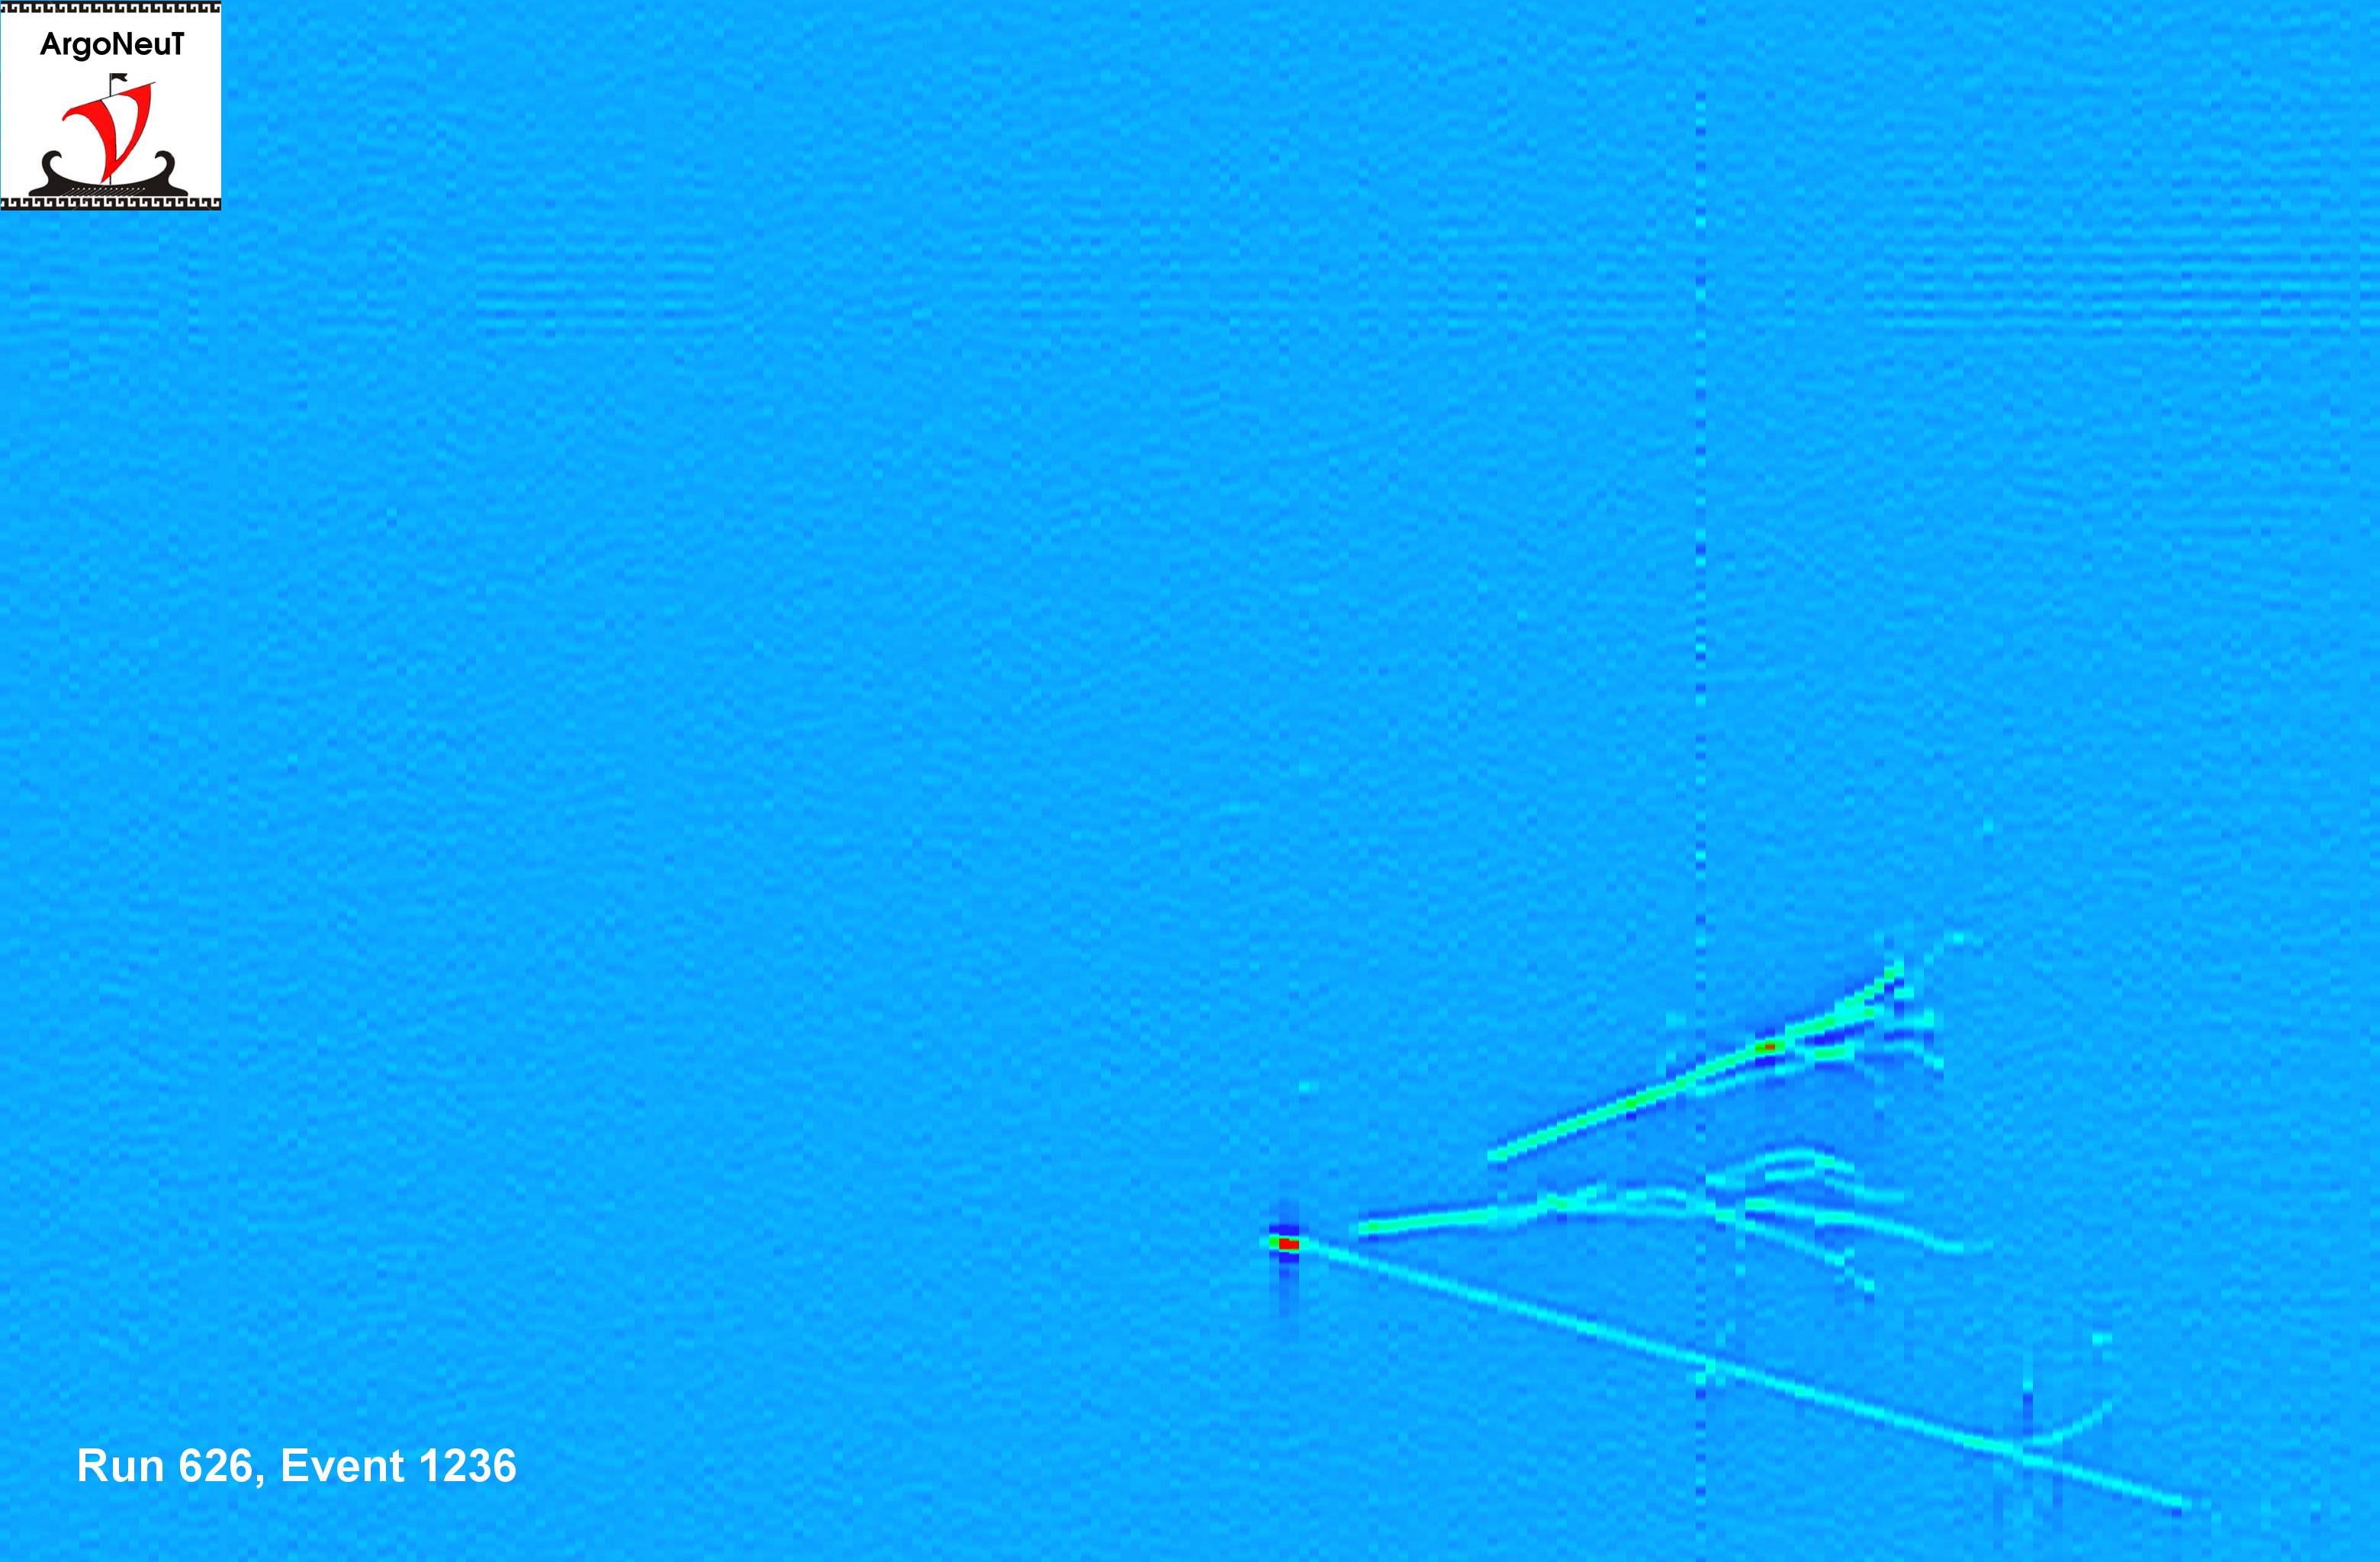
\includegraphics[width=0.85\textwidth]{lartpc_figures/R626_E1236_induction.png}
  \caption[\argoneut Event Images]{Full Resolution \argoneut data.  The horizontal direction, from left to right, represents increasing wire number.  The vertical direction is the drift distance, with the wires at the bottom of the picture.  An artificial color scale is applied to highlight depositions of charge above noise levels.  The top image is the collection plane, and the bottom image is the induction plane.  The wire signals here are deconvolved, which removes the bipolar shape of the induction pulse.}
  \label{fig:argoneut_data}
\end{figure}

\begin{figure}[htbp]
  \centering
  \includegraphics[width=\textwidth]{lartpc_figures/argoneut_plane_projection.pdf}
  \caption[\argoneut 3D projection]{Representation of the projection of the LArTPC in \argoneut.  The wire and time axes give a 2D image that represents a projection of the 3D charge depositions on to the 2D surfaces shown in blue.  Figure from \cite{Anderson:2012vc}.}
  \label{fig:argoneut_projection}
\end{figure}

\subsection{Deconvolution}
The reconstruction of these images into a 3D event starts at the lowest level, filtering and deconvolution of the wire signals.  In general, the number of electrons recorded by a given wire as a function of time is not perfectly matched by the ADC signals read out by the detector, due to the response of the detector electronics and noise effects.

To correct for this, a deconvolution process is applied to each wire.  As seen in figure \ref{fig:signal_shaping}, the response of the detector to a delta function introduces a spread of signal which is removed using a scheme with the Fast Fourier Transform. The response of each channel is measured with external pulse generators.  The convolution theorem then allows the removal of the detector response by taking the  inverse Fourier transform of $\frac{v[t]}{r[t]}$, where $v[t]$ is the Fourier transform of the recorded waveform and $r[t]$ is the Fourier transform of the channel's response.  Figure \ref{fig:argoneut_signals} shows the result of applying deconvolution to \argoneut data in the collection and induction planes.  In addition, the deconvolution for the induction plane removes the bipolar behavior to make hit finding easier.

\begin{figure}[htbp]
  \centering
  \includegraphics[width=\textwidth]{lartpc_figures/argoneut_signal_shaping.pdf}
  \caption[Signal Shaping in \argoneut]{On the left, an image of the idealized detector response to drift electrons in the induction and collection plane.  On the right, the response of the electrons filter and digitization to a delta function pulse.  Figure from \cite{Anderson:2012vc}.}
  \label{fig:signal_shaping}
\end{figure}


\subsection{Hit Finding}

For each wire in the detector, a hit finding algorithm is used to locate the regions of the readout with electron deposition signals.  While there are several different hit finding algorithms available in LArSoft \cite{Church:2013hea}, the official LArTPC reconstruction software, they all follow a generalized procedure.

First, a deconvolved (and noise filtered) wire signal is scanned for regions of signal above a specified threshold.  The baseline threshold of hit finding depends on whether the signal is from collection or induction planes, as the two planes have different Signal to Noise ratios.

Next, the regions of interest are fitted with an analytic function to allow a precise determination of the time tick, peak, and integral of the charge deposited.  The most common function used is a Gaussian.  In some cases, and commonly in neutrino interactions, hits that are close to each other from different particles will have overlapping regions.  In this case, the multiplicity of the region above threshold can be determined to help tracking algorithms accurately distribute hits between different particles.  An example of this is seen in Figure \ref{fig:argoneut_hit_multiplicity}.  In general, complicated regions with multiple hits are fit with several Gaussian functions summed together.

\begin{figure}[htbp]
  \centering
  \includegraphics[width=\textwidth]{lartpc_figures/argoneut_hit_multiplicity.pdf}
  \caption[Hit Finding in \argoneut]{A neutrino vertex as seen in the induction view in \argoneut.  The top left shows the reconstructed signals above threshold.  The other figures show the wire signal moving away from the vertex: the initial signal is wider than normal, and as the tracks diverge in the detector the two peaks are resolved.  Figure from \cite{Anderson:2012vc}.}
  \label{fig:argoneut_hit_multiplicity}
\end{figure}

\subsection{Cluster, Tracking and 3D Reconstruction}

Once the wire signals have been deconvolved, and the signal depositions have been reconstructed as hits, a number of higher level steps remain between hits and physics data.  First, hits must be grouped together based on which particle they originated from.  In general, this is an {\em extremely} difficult problem with no simple answer.  For particles like muons and protons, which produce simple, linear tracks of hits in the detector, it is not impossible and a lot of progress has been made.  For more complicated events, such as electromagnetic showers and deep inelastic scatter events, clustering remains the weakest point of the reconstruction chain.

For a track like particle, in general, the groups of hits are associated together into clusters by finding sets of hits that are well aligned linearly.  These clusters are then matched across the planes of the detector (two planes in \argoneut, but many state of the art detectors have 3).  Though the planes offer different projections of the 3D events into 2D, the drift direction (vertical direction in \ref{fig:argoneut_data}) is a common axis in every projection.  Therefore, the most useful metric to determine if two clusters are from the same track in the argon is the time it took those clusters to drift to the wires.

Once clusters from multiple planes have been matched together, the wire information between the two clusters can be used to determine where in the Y-Z plane the clusters overlap.  This is because each wire intersects the other plane's wires at most once, so if a charge deposition from one plane is matched to one on another plane, it uniquely determines the location of the 3D charge (The X coordinate comes from the drift time).

Almost all of the details of 3D tracking and reconstruction have been abbreviated here, as they are not crucial to the work presented in this thesis.  However, a great detail of knowledge and techniques is reported in many references \cite{Antonello:2012hu,uboone_pub_1015}.

%
% Edited up to here.
%

\subsection{\label{subsec:lartpc_calibration} Calibration}

For a \lartpc to perform physics studies with calorimetric information, it is essential to accurately calibrate the detector response to charge depositions on the wires.  For \argoneut, this was performed with large sample of crossing muons as reported in \cite{Anderson:2012mra}.  That analysis demonstrated that muons induced from upstream interactions (known as ``through-going muons'' in \argoneut) can be used as a known source of ionization in the detector, as shown in Figure~\ref{fig:mpv_muons}.  For \argoneut, the mean momentum of the through-going muons was estimated at 7 GeV/c.

\begin{figure}[tb]
  \centering
  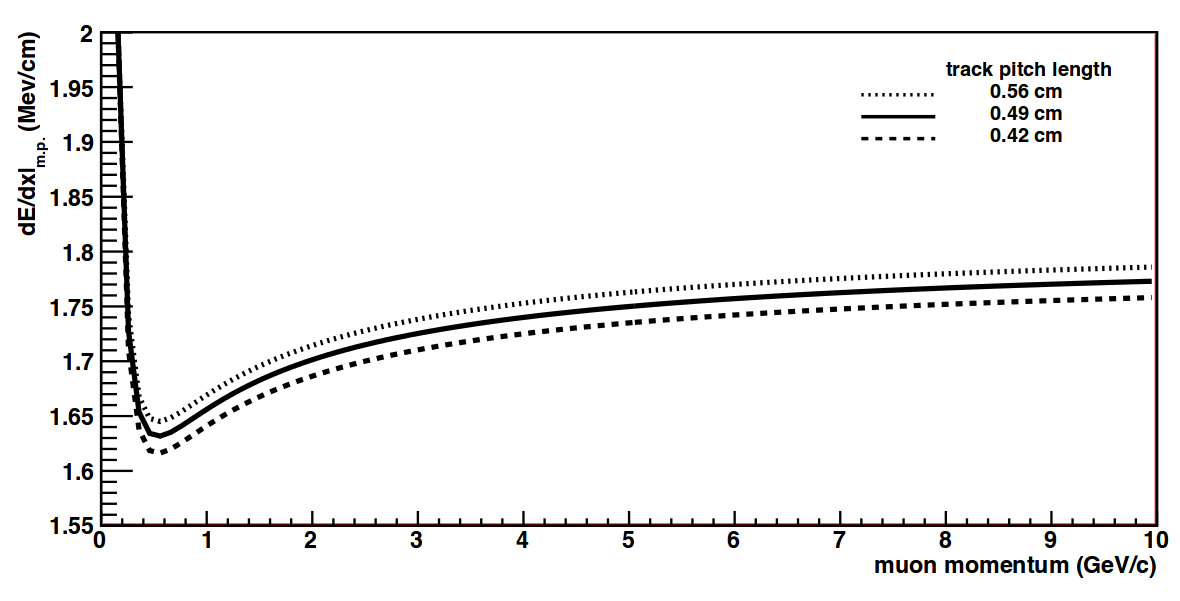
\includegraphics[width=\textwidth]{lartpc_figures/mpv_muons.png}
  \caption[Most Probable Ionization, Muons]{Most probable ionization amounts for muons traversing liquid Argon, as a function of momentum.}
  \label{fig:mpv_muons}
\end{figure}

To calibrate the detector from a sample of muons, the $dE/dx$ of each deposition measured by the wires of the TPC can be collected into a histogram and the shape is fit with a Gaussian-convolved Landau distribution, as demonstrated in Figure~\ref{fig:coll_mpv_muons}.  If the most probable value of the distribution, which is a parameter of the fit, is observed to be different from the target value (1.73 MeV/cm), the calibration constants are adjusted.  This process repeats until the calibration constant produces a distribution of hits that agrees with theoretical values of ionization per centimeter.

Unlike \cite{Anderson:2012mra}, there are two differences in the calibration used in the analyses described in Chapter~\ref{chp:emshowers}. First, the calibration constants are calculated on a wire-by-wire basis, instead of for the entire detector.  Second, the calibration constants are calculated for both the collection and the induction plane, instead of just the collection plane.  Due to advancements in deconvolution and hit finding since the original publication of the \argoneut calibrations, the induction plane can now be shown to be a usable plane for calorimetry, as seen in Figure~\ref{fig:coll_ind_differences}.  The two planes show agreement in the calorimetric values calculated for the crossing muons.  In the end, the average calibration constants for each plane are determined to be 36.4 $\pm$ 2.48 [fC/(ADC*tick)] for the collection plane, and 143 $\pm$ 10.3 [fC/(ADC*tick)].

\begin{figure}[tb]
  \centering
  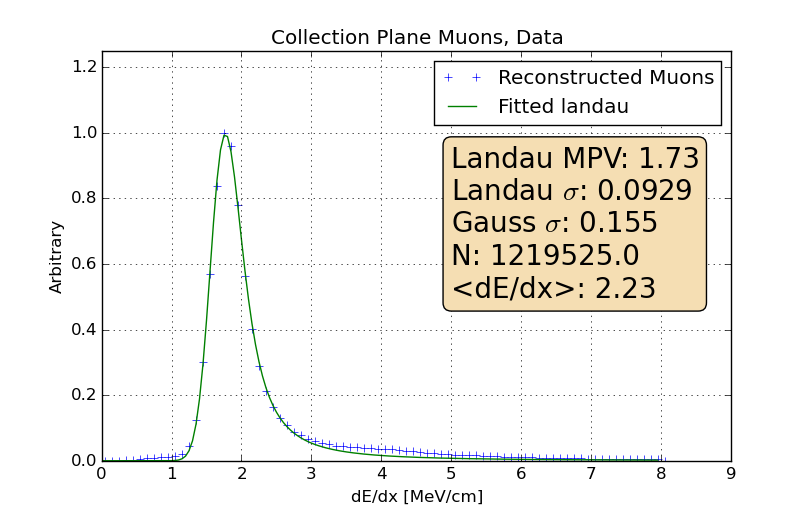
\includegraphics[width=0.45\textwidth]{lartpc_figures/collection_muons_total.png}
  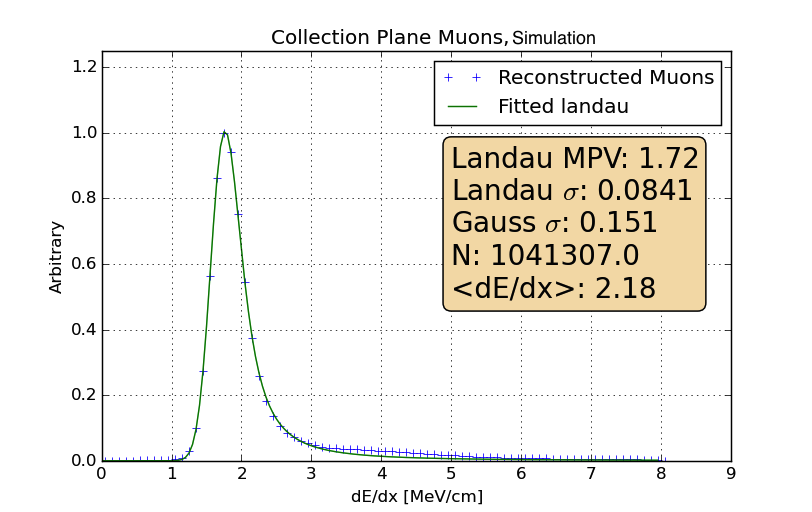
\includegraphics[width=0.45\textwidth]{lartpc_figures/collection_muons_total_sim.png}
  \caption[Muon $dE/dx$ Distributions]{Most probable ionization amounts for muons traversing liquid Argon, as a function of momentum.  Data are shown on the left, with simulation results on the right.}
  \label{fig:coll_mpv_muons}
\end{figure}

\begin{figure}[p]
  \centering
  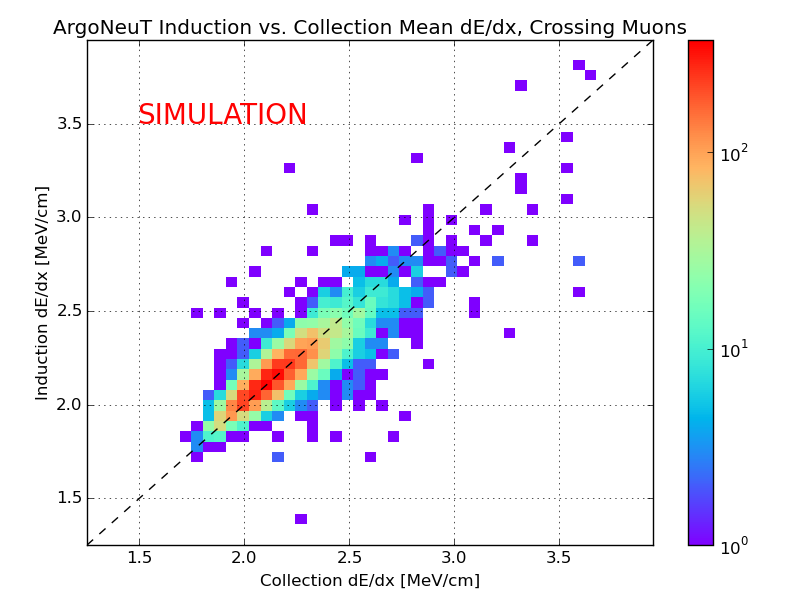
\includegraphics[width=0.45\textwidth]{lartpc_figures/mean_coll_vs_ind_sim_muons.png}
  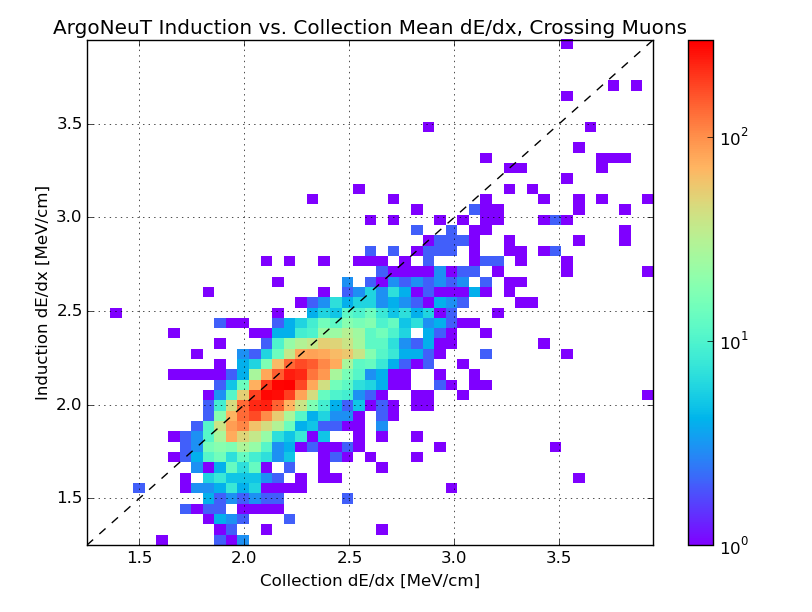
\includegraphics[width=0.45\textwidth]{lartpc_figures/mean_coll_vs_ind_data.png}
  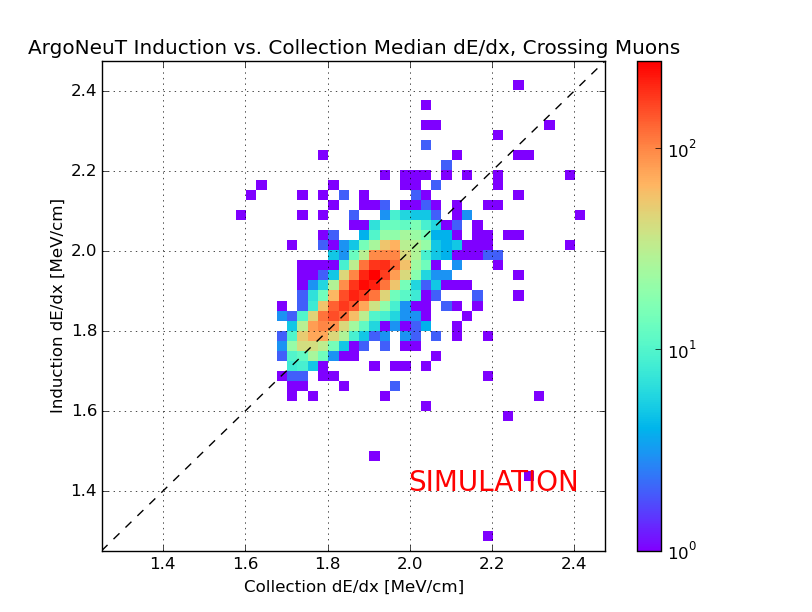
\includegraphics[width=0.45\textwidth]{lartpc_figures/median_coll_vs_ind_sim_muons.png}
  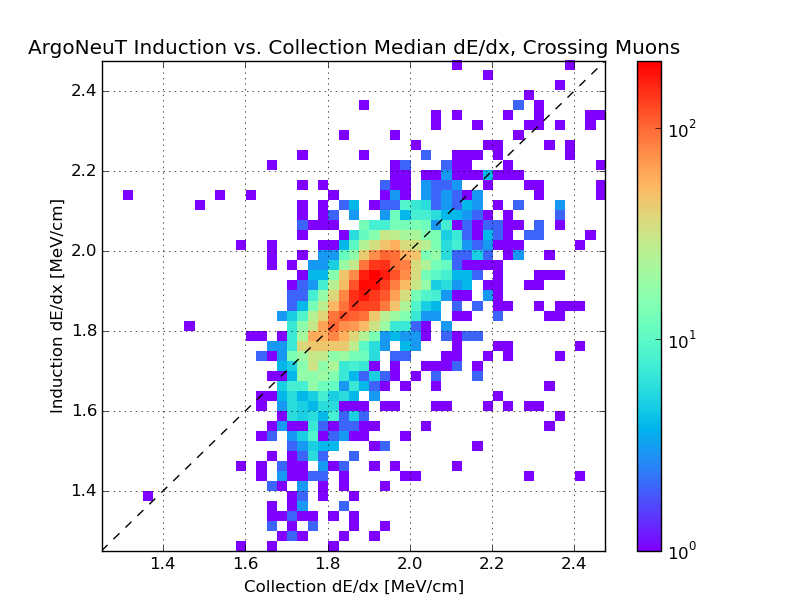
\includegraphics[width=0.45\textwidth]{lartpc_figures/median_coll_vs_ind_data.png}
  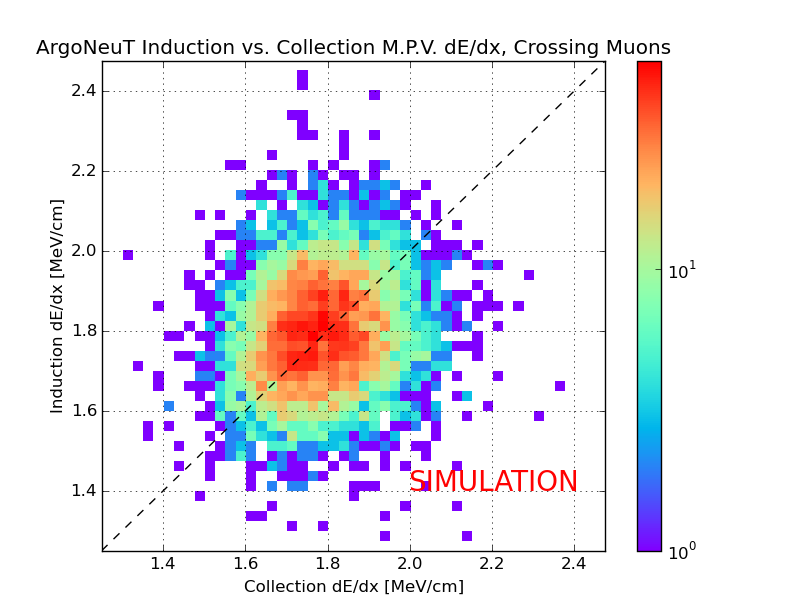
\includegraphics[width=0.45\textwidth]{lartpc_figures/mpv_coll_vs_ind_sim_muons.png}
  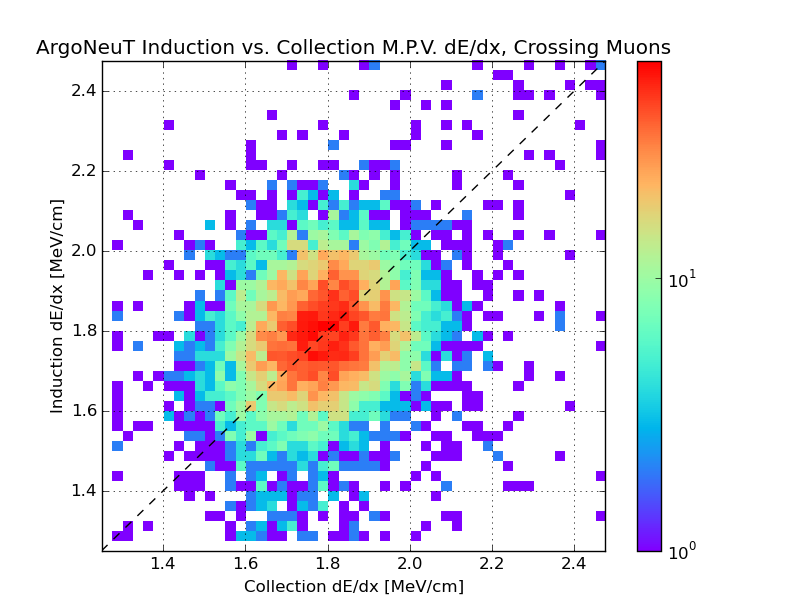
\includegraphics[width=0.45\textwidth]{lartpc_figures/mpv_coll_vs_ind_data.png}
  \caption[Cross Plane Calibration Checks]{A comparison of the mean, median, and most probable value for crossing muons between the collection (x axis) and induction (y axis) planes.  Simulation is shown on the left, data on the right.  There is good agreement between collection and induction planes, as well as between simulation and data.}
  \label{fig:coll_ind_differences}
\end{figure}

\subsection{Particle Identification and Calorimetry}

In a LArTPC, the calorimetric identification of particles is based upon the behavior of charged particles moving through the argon.  The energy deposited per centimeter is dictated by the Bethe-Bloch equations, and the properties in argon of common particles are seen in Figure \ref{fig:bethe_bloch}.

\begin{figure}[htbp]
  \centering
  \includegraphics[width=\textwidth]{lartpc_figures/mpv_particles}
  \caption[MPV Ionization in Argon for Common Species of Particles]{Most probable ionization per centimeter in argon for a variety of common particles.}
  \label{fig:bethe_bloch}
\end{figure}

As a particle loses energy, it's amount of ionization decreases until it reaches a minimum before the ionization spikes to very high values.  Due to the limited resolution of the detector, however, the observed $dE/dx$ values for a given particle will increase as the particle comes to a rest.  As seen in Figure \ref{fig:residual_range}, this measure of $dE/dx$ versus residual range allows calorimetric separation of particles.  In particular, protons are easily separated from muons and pions with this measure.

\begin{figure}[tb]
  \centering
  \includegraphics[width=\textwidth]{lartpc_figures/residual_range.pdf}
  \caption[Residual Range]{(Left) $dE/dx$ versus residual range of various particles in liquid Argon.  The values of $dE/dx$ vs. Residual range for a particle observed in the detector can be used to identify the particle's type. (Right) A stopping particle in the \argoneut detector.  The values of this particle's $dE/dx$ versus residual range (black points on left) identify it as a proton.}
  \label{fig:residual_range}
\end{figure}

Since LArTPCs also offer bubble chamber quality images, the topology of an event can give excellent ways to distinguish particles.  As seen in Figure \ref{fig:mu_pi}, particles like muons and pions that are difficult to distinguish with calorimetry can often be separated based on subsequent interactions within the TPC.

\begin{figure}[tb]
  \centering
  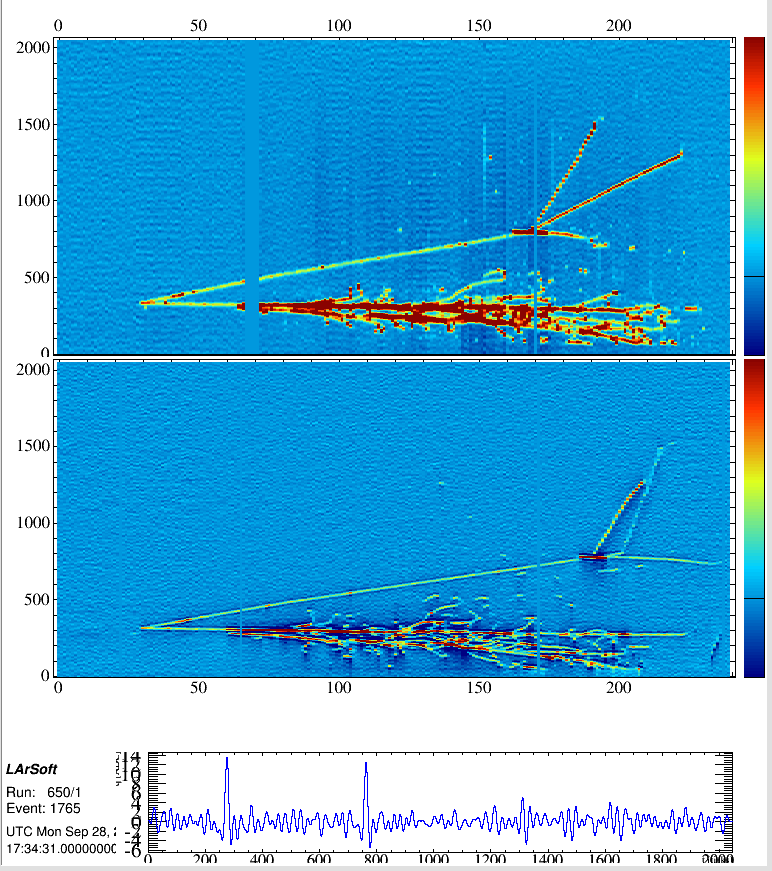
\includegraphics[width=\textwidth]{lartpc_figures/r650_1765_pi_zero_overlaid_with_track.png}
  \caption[Pion Reinteraction]{An \argoneut event with a strong pion reinteraction.  The pion track, starting from the bottom left and moving towards the top right, reinteracts with an argon nucleus through a hadronic interaction.  The resulting topology of many particles from the secondary interaction easily distinguishes this track as a pion and not a muon.}
  \label{fig:mu_pi}
\end{figure}



\subsection{MINOS}

\argoneut is fortunate in that it was located directly upstream of the MINOS near detector, which is a magnetized tracking detector \cite{Michael:2008bc}.  This gives \argoneut a distinct trait that no other LArTPC has had: muon sign selection for muons produced in \argoneut that enter the MINOS near detector.

\begin{figure}[htb]
  \centering
  \includegraphics[width=\textwidth]{lartpc_figures/minos.pdf}
  \caption[\argoneut and MINOS]{An event display depicting the \argoneut experiment and the MINOS near detector. \argoneut is the small box in the foreground.  The tracks represent TPC data of \numu CC interactions that were successfully tracked and matched into the MINOS near detector.  Figure from \cite{Anderson:2012vc}.}
  \label{fig:minos}
\end{figure}

\argoneut is only 90cm long at it's longest dimension, and since the NuMI beam has neutrino energies of 10+ GeV, it is extremely rare for muons produced in \argoneut to stop within the detector.  This enabled several precision measurements of muon neutrino cross sections on argon by looking for neutrinos that interact in \argoneut, and tracking them through the MINOS near detector \cite{Anderson:2011ce, Acciarri:2014isz}.

For the analyses presented in this thesis, MINOS is not used as a muon spectrometer directly.  Instead, since the target interaction is electron neutrinos, MINOS is able to provide rejection of muon neutrino events.

\FloatBarrier

\section{Current and Future \lartpcs}

\argoneut, the main subject of this chapter, was the first LArTPC in a neutrino beam in the U.S. and the start of the U.S. \lartpc neutrino program.  Before \argoneut even collected data, however, another \lartpc was already proposed: \uboone.  Since then, \lartpcs have become the detector of choice for neutrino physics in the ~GeV energy range.  This section describes some of the important future TPCs in the US neutrino program. 

\subsection{\label{sec:microboone} \uboone}

\uboone \cite{Chen:2007ae} is the successor to \MB \cite{AguilarArevalo:2008qa} (See Section~\ref{sec:miniboone}), and is designed to confirm or rule out the \MB ``Low Energy Excess,'' described further in Chapter~\ref{chp:sbn}.  \uboone is large TPC, 235 $ (w) \times $ 250 $ (h) \times $ 10.95 $ (l) $ m$^3$, or about 87 tons of Liquid Argon - see Figure~\ref{fig:uboone_det}.  The most notable differences, other than size, between \argoneut and \uboone are the third instrumented wire plane and the PMT system for light collection.  Additionally, the wire spacing in \uboone is 3~mm, decreased from 4~mm in \argoneut.

\begin{figure}[htb]
  \centering
  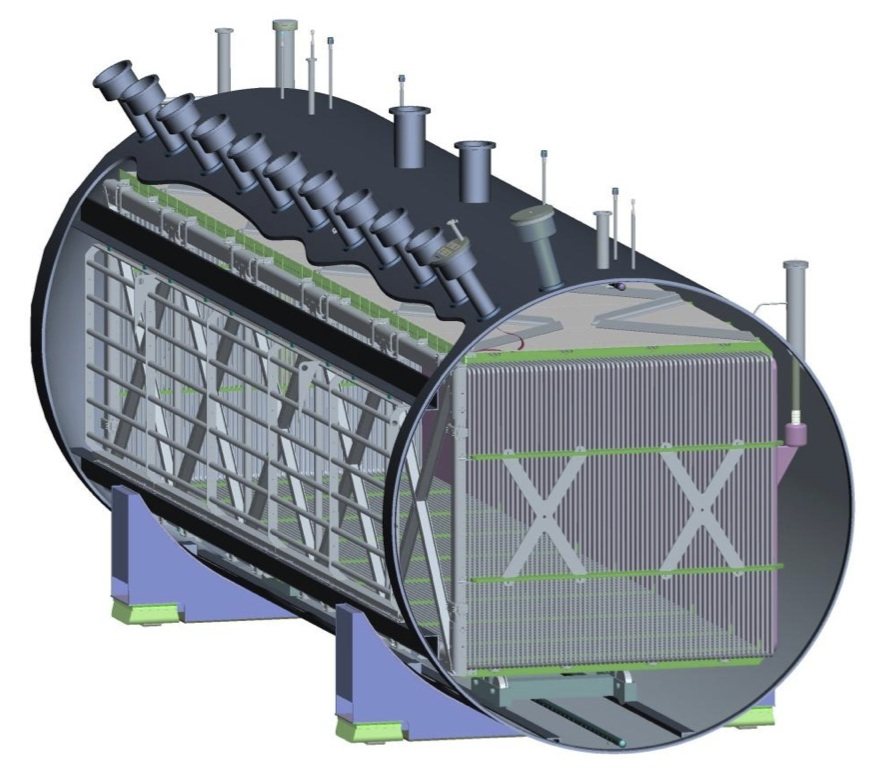
\includegraphics[width=0.5\textwidth]{lartpc_figures/uboone_tpc.jpg}
  \caption[\uboone Detector Design]{A schematic image of the \uboone detector as it was designed.  The beam enters from the bottom right side of the detector, along the longest axis.  The high voltage cathode is on the right, back of the detector while the sense wires are on the exposed left side where the cryostat has been cut away.}
  \label{fig:uboone_det}
\end{figure}

\uboone's main physics goal, the resolution of the Low Energy Excess, is in addition to a host of other physics and R\&D tasks.  On the physics side, \uboone will provide exceptional data for studying neutrino interactions, particularly in understanding nuclear physic effects in neutrino interactions.  \uboone has the finest 3D resolution of any calorimetric neutrino detector to date, allowing it to measure the outgoing hadrons (protons, pions, neutrons, kaons, etc.) from a neutrino interaction.  An image of the \uboone collection plane, Figure~\ref{fig:uboone_r3469_e28734}, showing a \numu candidate event with a proton and $\pi^0$, showcases \uboone's precision imaging.  \uboone expects high statistics in many interesting neutrino cross section channels, as shown in Table~\ref{tab:uboone_xsec}.  The cross section measurements of \uboone (and SBND and ICARUS) will be a major legacy of the Fermilab \lartpcs especially in the DUNE\cite{DUNE} era.


\begin{figure}[htb]
  \centering
  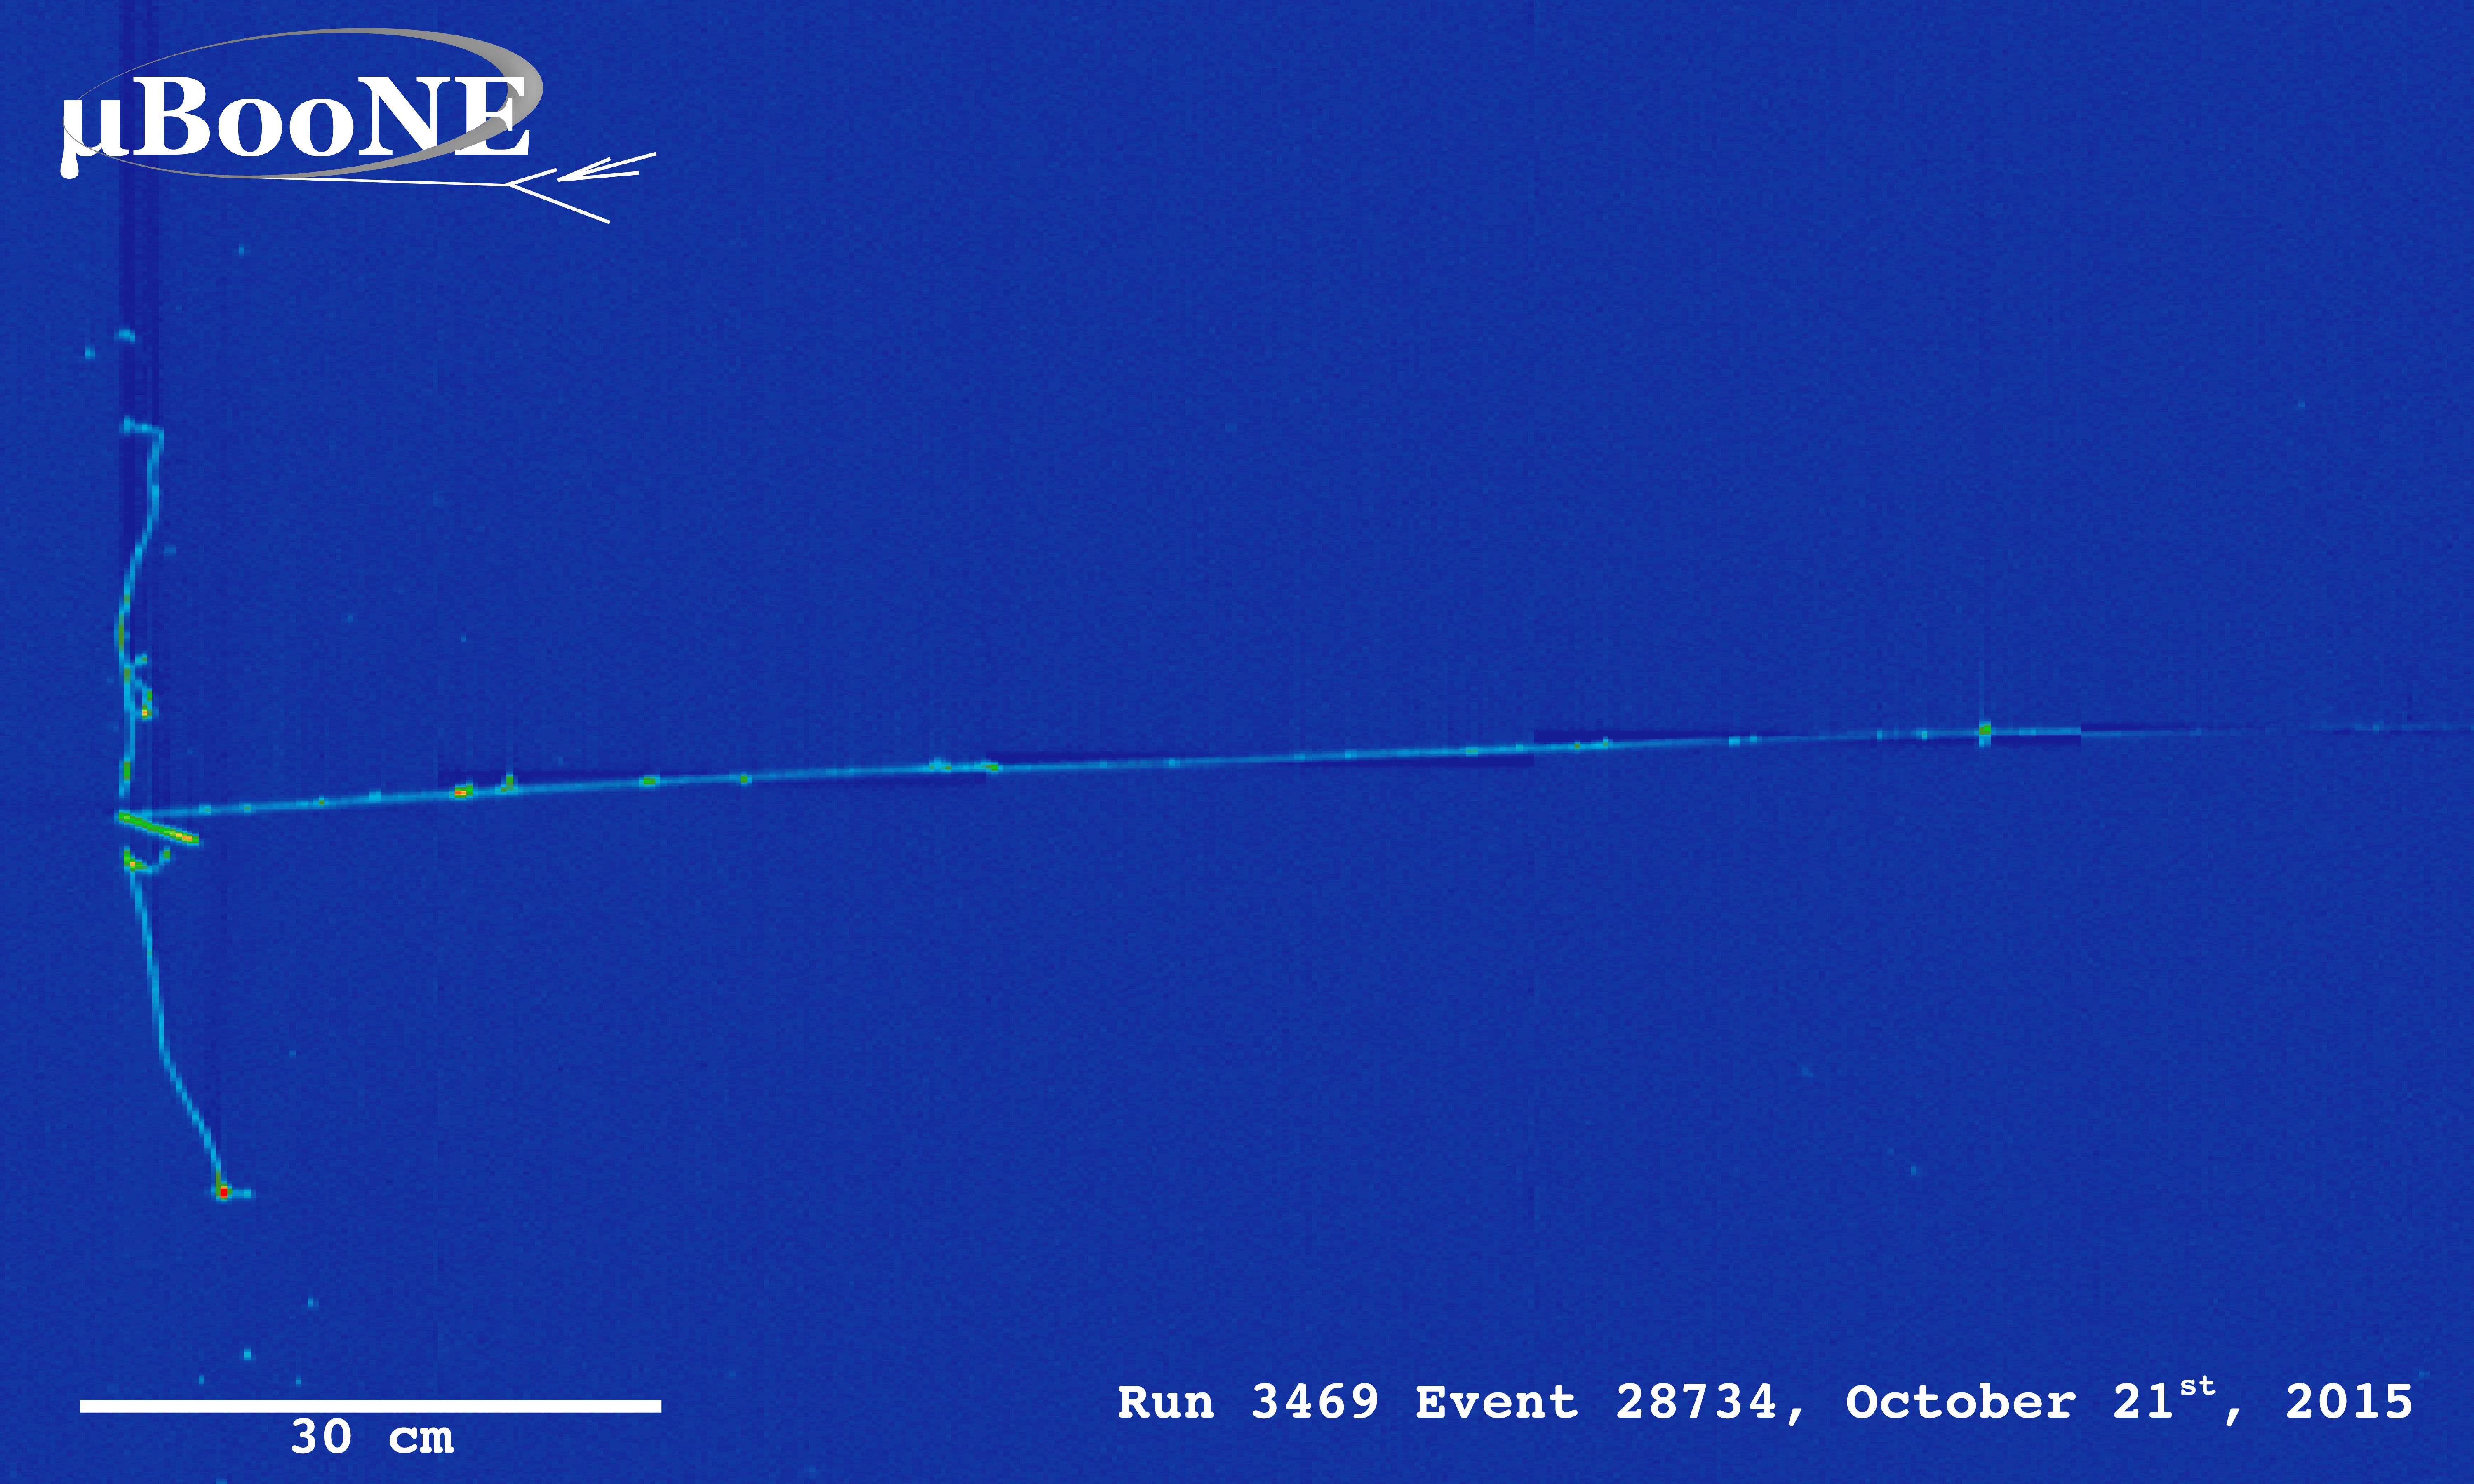
\includegraphics[width=0.75\textwidth]{lartpc_figures/run3469_subrun574_event28734_col_small.png}
  \caption[\uboone Run 3469, Event 28734]{}
  \label{fig:uboone_r3469_e28734}
\end{figure}

\begin{table}[htbp]
  \centering
  \begin{tabular}{l c r}
    {\bf Process}  & \hfill & {\bf No. Events} \\
    \hline
    \hline
    \multicolumn{3}{c}{\numu Events by Topology} \\
     & & \\
    CC Inclusive & & 122,100 \\
    CC 0 $\pi$  & \numu N $\rightarrow \mu$ + Np & 78,500 \\
      & ~$\cdot$ \numu N $\rightarrow \mu$ + 0p & 16,500 \\ 
      & ~$\cdot$ \numu N $\rightarrow \mu$ + 1p & 44,200\\
      & ~$\cdot$ \numu N $\rightarrow \mu$ + 2p & 8,300\\
      & ~$\cdot$ \numu N $\rightarrow \mu$ + $\ge$ 3p & 9,500\\
    CC 1 $\pi^\pm$ & \numu N $\rightarrow \mu$ + nucleons + 1$\pi^\pm$ & 30,300 \\
    CC $\ge$ 2 $\pi^\pm$ & \numu N $\rightarrow \mu$ + nucleons + $\ge$ 2 $\pi^\pm$ & 2,700 \\
    CC $\ge$ 1 $\pi^0$ & \numu N $\rightarrow \mu$ + nucleons + $\ge$ 1 $\pi^0$ & 13,400 \\
    & & \\
    NC Inclusive & & 45,900 \\
    NC 0 $\pi$ & \numu N $\rightarrow \mu$ + nucleons & 29,900 \\
    NC 1 $\pi^\pm$ & \numu N $\rightarrow \mu$ + nucleons + 1$\pi^\pm$ & 6,900 \\
    NC $\ge$ 2 $\pi^\pm$ & \numu N $\rightarrow \mu$ + nucleons + $\ge$ 2 $\pi^\pm$ & 900 \\
    NC $\ge$ 1 $\pi^0$ & \numu N $\rightarrow \mu$ + nucleons + $\ge$ 1 $\pi^0$ & 9,200 \\
    \hline
    \hline
    \multicolumn{3}{c}{\nue Events} \\
    CC Inclusive & & 820 \\
    NC Inclusive & & 290 \\
    \hline
    \hline
  \end{tabular} 
  \caption[\uboone Event Rates]{Estimated event rates using GENIE (v2.8) in a 6.6e20 POT exposure of MicroBooNE, located 470m from the neutrino source, the Booster Neutrino Beam. In enumerating proton multiplicity, there is a kinetic energy threshold on protons of 20 MeV. The 0$\pi$ topologies include any number of neutrons in the event. This study uses a 17cm fiducial volume cut in MicroBooNE, which gives a fiducial volume of 61t.}
  \label{tab:uboone_xsec}
  
\end{table}

\uboone also introduces a number of important R\&D acheivements to the field of \lartpcs.  It is the first large scale \lartpc to acheive high purity without evacuating the cryostat.  Instead, the TPC used a purge of high purity argon gas to push impurities out of the cryostat before colling the cryostat and filling with liquid argon.   In this way, critical impurities were removed from the detector - see Figure~\ref{fig:o2purge}.  Additionally, \uboone employs cold readout electronics immersed in the liquid argon.  As seen in Figure~\ref{fig:noise_vs_temp}, the average noise level of the readout wires decreased dramatically during the cooldown of the \uboone cryostat.

\begin{figure}[htb]
  \centering
  \includegraphics[width=0.75\textwidth]{lartpc_figures/O2Purge.pdf}
  \caption[\uboone O2 Contamination]{The oxygen contamination of the gaseous argon while purging air. The sensor for this oxygen concentration was turned on after 10:00 AM April 21, 2015, and it reached its sensitivity limit during the evening of April 23, 2015. \cite{uboone_pub_1003}}
  \label{fig:o2purge}
\end{figure}


\begin{figure}[htb]
  \centering
  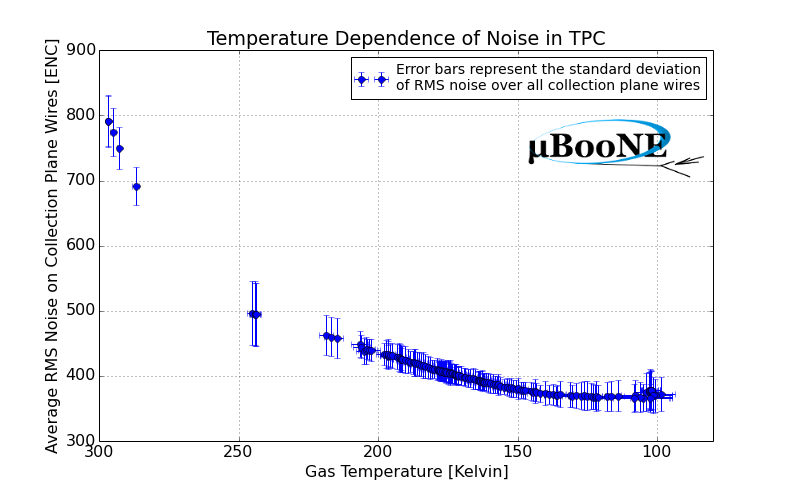
\includegraphics[width=0.45\textwidth]{lartpc_figures/noise_vs_temp.png}
  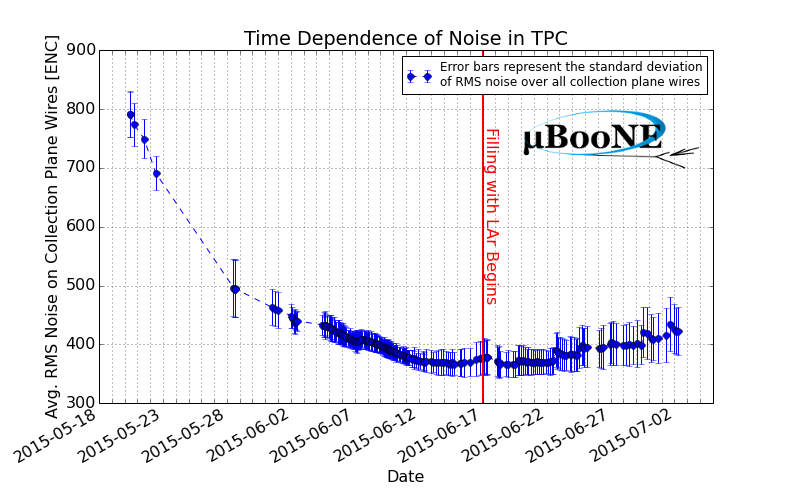
\includegraphics[width=0.45\textwidth]{lartpc_figures/noise_vs_time.png}
  \caption[\uboone Noise Temperature Dependence]{Noise measured on collection plane wires as a function of temperature (left) and time (right).  Data points represent the average RMS, and error-bars show the standard deviation of these distributions. Error bars are meant to show how the change in temperature affects noise levels compared to the intrinsic variability of noise in the detector due to channel-to-channel gain variations. \cite{uboone_pub_1001} }
  \label{fig:noise_vs_temp}
\end{figure}

Another significant improvement that \uboone brings that \argoneut did not have is the addition of a light collection system.  A light collection system is essential for detectors like \uboone running on the surface and not deep underground.  The \uboone light collection is composed of 8 inch Photo-Multiplier Tubes (PMTs) arrayed behind the wire planes.  Argon scintillates at a vacuum ultraviolet wavelength (to which liquid argon is transparent), but the PMTs detect visible light.  So, each PMT has a wavelength shifting plate to convert the vacuum ultra violet to visible light detectable by the PMTs.

On the surface, \uboone is exposed to a high flux of cosmic rays, as many as ~10 cosmic ray interactions in the detector each readout window of 4.8 ms.  On the other hand, the detector is exposed to the neutrino beam for just several $\mu$s.  Though the wire information can not be used to identify precisely when an interaction occurred in the TPC, the PMT information detects flashes of light with each particle interaction and can localize interactions in a much tighter region of time.  This provides two advantages: first, if the time of an interaction is known (particularly cosmic interactions), the corrections that must be applied as a function of drift distance (such as lifetime corrections) can be accurately applied.  Second, and more important for a successful operation of the detector, the PMT system provides a triggering system for the beam interactions, as shown in Figure~\ref{fig:pmt_timing}.  A clear excess of PMT flashes coincident with the expect neutrino beam, for both BNB and NuMI beams, can be seen.  By only saving events to disk when there is a PMT flash in this region of time, \uboone is able to dramatically reduce it's consumption of network bandwidth and disk storage.

\begin{figure}[htb]
  \centering
  \includegraphics[width=0.45\textwidth]{lartpc_figures/BNB_pmt_timing.pdf}
  \includegraphics[width=0.45\textwidth]{lartpc_figures/NUMI_pmt_timing.pdf}
  \caption[\uboone O2 Contamination]{The measured distribution of flash times (requiring flashes greater than 50PE) with respect to the trigger time for BNB-triggered events (left) and NuMI-triggered events (right), shown as a ratio to the expected cosmic rate from off-beam data. The blue band denoting the cosmic rate was centered at one, with a width corresponding to the measured uncertainty in the cosmic rate. A clear excess can be seen due to neutrinos between 3 and 5 $\mu$s (for BNB) 6 and 15 $\mu$s (for NuMI) after the trigger. This is where the neutrinos were expected based on the Resistive Wall Monitor signal arrival time. A total of 1.92E6 BNB (left) and 3.67E5 NuMI (right) triggered events (unbiased trigger) were used to produce this plot. \cite{uboone_pub_1010}}
  \label{fig:pmt_timing}
\end{figure}

\uboone began taking neutrino data in the fall of 2015, and collected approximately 3.5E20 POT (about half of its data set) by the fall of 2016.  In the near future, \uboone will determine the origin of \MB's low energy excess.  \uboone will lead the Fermilab Short Baseline Program forward as the first running \lartpc on the Booster Neutrino Beam, which is an exciting step forward in the U.S. \lartpc program.

\FloatBarrier

\subsection{\label{sec:future_tpcs} Future LArTPCs}

As mentioned above, \uboone is the newest \lartpc to the Fermilab Short Baseline Program, but there are two other \lartpcs planned to begin operation within several years.  In this brief section, I will give a few selected details of these other two detectors as they are both critical components of the SBN program and essential to resolving short baseline neutrino anamolies (see Chapter~\ref{chp:sbn}).

\subsubsection{\label{subsec:sbnd} SBND}

Along the Booster Neutrino Beam, SBND will be the \lartpc closest to the neutrino source.  It is currently under design and construction, with final assembly taking place in 2017 and 2018.  Due to the proximity of SBND to the BNB target and the high power of the BNB, SBND will have the highest statistics measurements of neutrino interactions of any \lartpc to date.  With over 1 million events per year, SBND records statistics equivalent to the \uboone data set in just one month (and it matches the statistics of \argoneut in just one day!).  With this expected event rate, SBND can probe rare neutrino interactions with high statistics.  The high event rate also allows precision measurements of final state topologies of neutrino interactions, which in turn is essential for tuning neutrino interaction models for DUNE.

Like \uboone, SBND will feature a light collection system to trigger neutrino events and accurately determine cosmic timing.  Unlike \uboone, SBND is a dual drift TPC with the high voltage cathode in the middle of the TPC, and two sets of read out wires on each side - see Figure~\ref{fig:sbnd_det}.  Like \uboone, SBND is driving forward the U.S. \lartpc program with important R\&D tasks, including the manufacture of Cathode Plane Assemblies and Anode Plane Assemblies.

\begin{figure}[htb]
  \centering
  \includegraphics[width=0.45\textwidth]{lartpc_figures/sbnd_cryostat.pdf}
  \includegraphics[width=0.45\textwidth]{lartpc_figures/sbnd_tpc.pdf}
  \caption[\sbnd Design]{The SBND TPC (left) and cryostat design (right).}
  \label{fig:sbnd_det}
\end{figure}

% Details of SBND, PMTS, proximity to beam, flux window, etc.

\subsubsection{\label{subsec:icarus} \icarus}

ICARUS is an international \lartpc that was run in Italy, and the first large scale \lartpc in a neutrino beam.  The detector, known as T600, is approximately 476 tons of active argon divided into two modules (known as T300 each).  The two modules were deployed together at Gran Sasso lab in Italy, underground, where they were exposed to CERN's CNGS neutrino beam.  ICARUS has been a pioneer of \lartpc technology.

After the CNGS beam was decommissioned, it was decided to transport the ICARUS detector from Italy to Fermilab for use as the third detector in the SBN Program.  ICARUS is significantly more massive than both \uboone and SBND, and so it offers the chance to record oscillation spectra from anomalous neutrino oscillations at a different L/E than \uboone, with high statistics.  Currently, ICARUS is at CERN where it is being refurbished and upgraded, before it is shipped to Fermilab for installation.

\begin{figure}[htb]
  \centering
  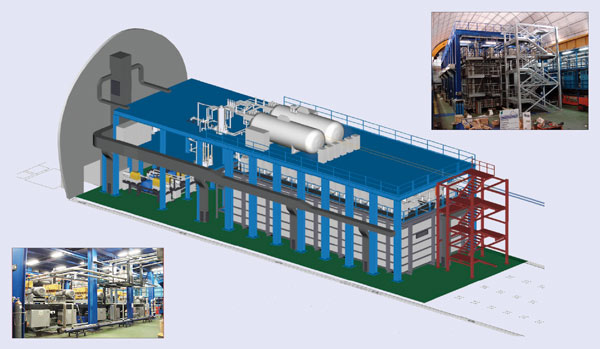
\includegraphics[width=0.45\textwidth]{lartpc_figures/icarus.jpg}
  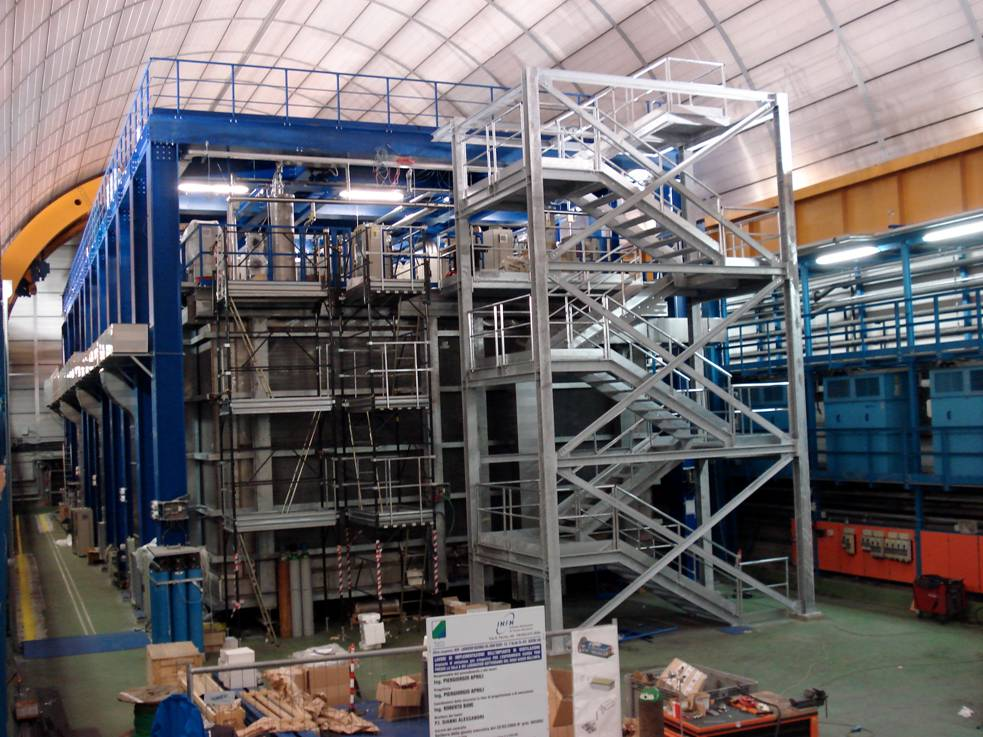
\includegraphics[width=0.45\textwidth]{lartpc_figures/icarus_real.png}
  \caption[ICARUS T600]{The design of the ICARUS T600 detector (left) and the realization of the detector underground at Gran Sasso lab in Italy (right).}
  \label{fig:icarus}
\end{figure}


\FloatBarrier

